\section{Visualisation des données}
Une page de visualisation des données a été crée en utilisant les langanges HTML, CSS, PHP, JavaScript et une librairie, ChartJS, permettant la création de graphique. Sur cette page on retrouve par exemple toutes les informations concernant un noeud, toutes les informations sur les capteurs  et les données relevées, représentées par des graphiques la figure \ref{fig:Page de visualisation des données}.
Une des améliorations a apporter à la visualisation, serait de pouvoir croiser les données pour pourvoir permettre une comparaison rapide des relevés capteurs. En effet, pour l'instant, pour une même donnée \begin{math}x \end{math} (exemple : température de l'aire) mesurée par deux capteurs distincts \begin{math}C_{1}\end{math} et \begin{math}C_{2}\end{math}, on a deux graphiques distincts, ces derniers étant construits par capteurs. Le but serait donc de combiner les deux graphiques en un seul graphique ce qui permettrait une comparaison plus rapide.
Ci-dessous, le code JavaScprit permettant la création des graphiques.
\begin{minted}{javascript}
function drawChart() {
    //accès aux données de la base via php par AJAX
    $.ajax({
        url:"../php/gestionnaire/dataHandler.php",
        type : "POST",
        data: ({idcapteurs:countSelectedCapteurs,
            date_debut:date_debut ,date_fin : date_fin}),
        success : function (data) {
            // boucle sur les données
            for(var i in data){
                var div_id="#chart"+data[i]['id_capteur'];
                var ctx = $(div_id);
                var chardata;
                var grandeurs = data[i]['grandeurs'];
                var datasets_tab = [];
                var labels_tab = [];

                for(var j in grandeurs){
                    var data_tab = [];
                    donnees = grandeurs[j]['donnees'];
                    if(labels_tab.length == 0){
                        for(var k in donnees){
                            // on place les date en Abscisse
                            labels_tab.push(moment(donnees[k]['date']).
                            format('MM Do YY, h:mm'));
                        }
                    }
                    // récupération des différents relevées
                    for(var k in donnees){
                        data_tab.push(parseFloat(donnees[k]['valeur']));
                    }

                    //construction des datasets
                    datasets_tab[j] = {
                        label : grandeurs[j]['label'].trim(),
                        borderColor : getRandomColor(),
                        fill : false,
                        data : data_tab
                    };

                };
                // création du graphique
                var chardata = {
                    labels : labels_tab,
                    datasets : datasets_tab
                };
                // construction du graphique sur la page html
                // librairie ChartJS
                window.myChart = new Chart(ctx,{
                    type : 'line',
                    data : chardata
                })
            }
        },
        error : function (data) {
            console.log("Erreur : Les données n'ont pas pu être récupérées");
        }
    });
};
\end{minted}
\begin{figure}
    \centering
    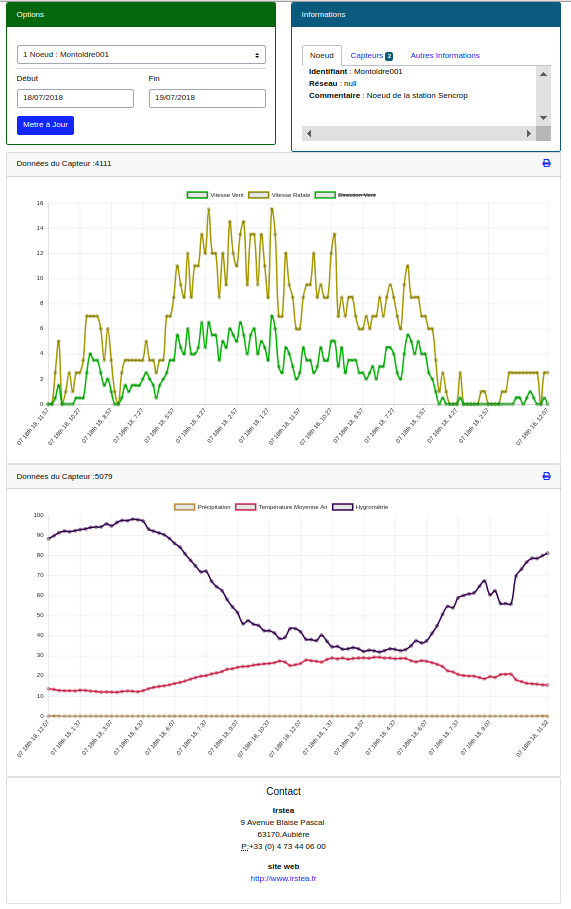
\includegraphics[height=.9\textheight]{images/db_visualisation.png}
    \caption{Page de visualisation des données}
    \label{fig:Page de visualisation des données}
\end{figure}


